% =========================================================
%  ppt/08-pathfinding-astar.tex
%  Materi 8 — Pathfinding Grid: dari BFS/Dijkstra ke A*
%  Bab X buku ajar
% =========================================================
\documentclass[aspectratio=169,10pt]{beamer}
% =========================================================
%  ppt/config/packages.tex
%  Paket bersama untuk seluruh presentasi kuliah
%  Pengantar Pemrograman Game
% =========================================================

\usepackage[T1]{fontenc}
\usepackage[utf8]{inputenc}
\usepackage[indonesian]{babel}
\usepackage{lmodern}
\usepackage{textcomp}
\usepackage{amsmath}
\usepackage{amssymb}
\usepackage{graphicx}
\usepackage{booktabs}
\usepackage{tabularx}
\usepackage{array}
\usepackage{multicol}
\usepackage{listings}
\usepackage{upquote}
\usepackage{adjustbox}
\usepackage{tcolorbox}
\usepackage{tikz}
\usetikzlibrary{
  arrows.meta,
  positioning,
  shapes.geometric,
  shapes.misc,
  calc,
  fit,
  backgrounds,
  matrix,
  chains,
  decorations.pathreplacing,
  patterns
}

\tcbuselibrary{skins}

% Jangan memuat geometry: ukuran halaman diatur oleh beamer.

% =========================================================
%  ppt/config/theme.tex
%  Satu tema Beamer untuk keempat belas presentasi
%  Pengantar Pemrograman Game
% =========================================================

% --------------------------------------------------------- warna
\definecolor{ubNavy}{HTML}{1F3864}
\definecolor{ubAccent}{HTML}{2E75B6}
\definecolor{ubHead}{HTML}{D9E2F3}
\definecolor{ubSoft}{HTML}{F2F6FC}
\definecolor{ubLine}{HTML}{BFBFBF}
\definecolor{ubText}{HTML}{1F2937}
\definecolor{ubMuted}{HTML}{5A6678}
\definecolor{ubGreen}{HTML}{1E7B45}
\definecolor{ubGreenBg}{HTML}{F1F8F2}
\definecolor{ubRed}{HTML}{B3261E}
\definecolor{ubRedBg}{HTML}{FDF2F1}
\definecolor{ubWarn}{HTML}{A35A05}
\definecolor{ubWarnBg}{HTML}{FFF8EC}
\definecolor{ubGray}{HTML}{F6F6F6}
\definecolor{ubCodeBg}{HTML}{10233F}
\definecolor{ubCodeText}{HTML}{E8EEF7}
\definecolor{ubCodeKey}{HTML}{8FBCF0}
\definecolor{ubCodeCom}{HTML}{8FB37A}
\definecolor{ubCodeStr}{HTML}{D9A46B}
\definecolor{ubCodeNum}{HTML}{7E99BE}

% Nama warna yang dipakai gambar TikZ buku ajar.
\definecolor{ubPrimary}{HTML}{1F3864}
\definecolor{ubAlt}{HTML}{F2F6FC}

% --------------------------------------------------------- dasar
\usetheme{default}
\usefonttheme{professionalfonts}
\setbeamertemplate{navigation symbols}{}
\setbeamerfont{frametitle}{size=\Large,series=\bfseries}
\setbeamerfont{framesubtitle}{size=\small}
\setbeamerfont{footline}{size=\tiny}
\setbeamerfont{block title}{size=\small,series=\bfseries}
\setbeamerfont{block body}{size=\small}
\setbeamerfont{itemize/enumerate body}{size=\small}
\setbeamerfont{itemize/enumerate subbody}{size=\footnotesize}

\setbeamersize{text margin left=0.60cm,text margin right=0.60cm}
\uchyph=0

\setbeamercolor{normal text}{fg=ubText,bg=white}
\setbeamercolor{structure}{fg=ubAccent}
\setbeamercolor{frametitle}{fg=ubNavy,bg=white}
\setbeamercolor{title}{fg=ubNavy}
\setbeamercolor{footline}{fg=ubMuted,bg=white}
\setbeamercolor{itemize item}{fg=ubAccent}
\setbeamercolor{itemize subitem}{fg=ubAccent}
\setbeamercolor{block title}{fg=white,bg=ubNavy}
\setbeamercolor{block body}{fg=ubText,bg=ubSoft}
\setbeamercolor{block title alerted}{fg=white,bg=ubWarn}
\setbeamercolor{block body alerted}{fg=ubText,bg=ubWarnBg}
\setbeamercolor{block title example}{fg=white,bg=ubGreen}
\setbeamercolor{block body example}{fg=ubText,bg=ubGreenBg}
\setbeamercolor{caption name}{fg=ubMuted}

\setbeamertemplate{blocks}[rounded][shadow=false]
\setbeamertemplate{itemize item}{\raisebox{0.10em}{\color{ubAccent}\scriptsize$\blacksquare$}}
\setbeamertemplate{itemize subitem}{\raisebox{0.06em}{\color{ubAccent}\tiny$\blacktriangleright$}}
\setbeamertemplate{enumerate item}{%
  \makebox[1.3em][l]{\color{ubAccent}\insertenumlabel.}}

\addtobeamertemplate{itemize/enumerate body begin}{%
  \setlength{\itemsep}{0.42em}\setlength{\parskip}{0pt}}{}

% --------------------------------------------------------- judul frame
\setbeamertemplate{frametitle}[default][left]

% --------------------------------------------------------- kaki
\newcommand{\materino}{00}
\newcommand{\materifoot}{Pengantar Pemrograman Game \textperiodcentered\ Materi \materino}

\setbeamertemplate{footline}{%
  \begin{beamercolorbox}[wd=\paperwidth,ht=0.015cm,dp=0cm]{footline}%
    \color{ubHead}\rule{\paperwidth}{0.4pt}%
  \end{beamercolorbox}%
  \begin{beamercolorbox}[wd=\paperwidth,ht=0.40cm,dp=0.14cm,%
                         leftskip=0.60cm,rightskip=0.60cm]{footline}%
    \usebeamerfont{footline}\color{ubMuted}\materifoot\hfill\insertframenumber%
  \end{beamercolorbox}%
}

% --------------------------------------------------------- makro buku ajar
\providecommand{\code}[1]{\texttt{\detokenize{#1}}}
\providecommand{\istilah}[1]{\emph{#1}}
\providecommand{\CPMK}[1]{CPMK\,#1}
\providecommand{\CPL}[1]{CPL\,#1}
\providecommand{\SUBCPMK}[1]{Sub-CPMK\,#1}

% --------------------------------------------------------- gaya kode
\lstdefinelanguage{CSharp}{
  morekeywords={abstract,as,base,bool,break,byte,case,catch,char,class,const,
    continue,decimal,default,delegate,do,double,else,enum,event,explicit,
    extern,false,finally,fixed,float,for,foreach,goto,if,implicit,in,int,
    interface,internal,is,lock,long,namespace,new,null,object,operator,out,
    override,params,private,protected,public,readonly,ref,return,sbyte,
    sealed,short,sizeof,stackalloc,static,string,struct,switch,this,throw,
    true,try,typeof,uint,ulong,unchecked,unsafe,ushort,using,virtual,void,
    volatile,while,var,get,set},
  sensitive=true,
  morecomment=[l]{//},
  morecomment=[s]{/*}{*/},
  morestring=[b]",
}

\lstdefinestyle{kode}{
  basicstyle=\ttfamily\footnotesize\color{ubCodeText},
  keywordstyle=\color{ubCodeKey}\bfseries,
  commentstyle=\color{ubCodeCom}\itshape,
  stringstyle=\color{ubCodeStr},
  numberstyle=\tiny\color{ubCodeNum},
  numbers=left,
  numbersep=7pt,
  backgroundcolor=\color{ubCodeBg},
  frame=none,
  showstringspaces=false,
  breaklines=false,
  tabsize=4,
  columns=fullflexible,
  keepspaces=true,
  xleftmargin=12pt,
  xrightmargin=2pt,
  aboveskip=0pt,
  belowskip=0pt,
  upquote=true,
}
\lstset{style=kode}

\newcommand{\kodejelas}[1]{%
  \vspace{0.16cm}%
  {\footnotesize\color{ubMuted}#1\par}%
}
\newcommand{\sumber}[1]{%
  \vspace{0.08cm}%
  {\scriptsize\color{ubMuted}\itshape #1\par}%
}
\newcommand{\awalan}[1]{%
  {\small\color{ubMuted}#1\par}\vspace{0.18cm}%
}

% --------------------------------------------------------- kotak
\newtcolorbox{kotak}[1][]{enhanced, colback=ubSoft, colframe=ubAccent,
  boxrule=0pt, leftrule=2.2pt, arc=1pt, left=6pt, right=6pt, top=4pt,
  bottom=4pt, fontupper=\footnotesize, #1}
\newtcolorbox{peringatan}[1][]{enhanced, colback=ubWarnBg, colframe=ubWarn,
  boxrule=0pt, leftrule=2.2pt, arc=1pt, left=6pt, right=6pt, top=4pt,
  bottom=4pt, fontupper=\footnotesize, #1}
\newtcolorbox{kiat}[1][]{enhanced, colback=ubGreenBg, colframe=ubGreen,
  boxrule=0pt, leftrule=2.2pt, arc=1pt, left=6pt, right=6pt, top=4pt,
  bottom=4pt, fontupper=\footnotesize, #1}

% --------------------------------------------------------- sampul
% \deckcover{nomor}{minggu}{judul}{sub-cpmk}{teknologi}{sumber}{blok}
\newcommand{\deckcover}[7]{%
\begin{frame}[plain]
\begin{tikzpicture}[remember picture, overlay]
  \fill[ubNavy] (current page.south west) rectangle ([xshift=6.00cm]current page.north west);
  \fill[ubAccent] ([xshift=6.00cm]current page.south west) rectangle ([xshift=6.08cm]current page.north west);

  \node[anchor=north west, text width=4.72cm, align=left, inner sep=0pt]
    at ($(current page.north west)+(0.66cm,-0.60cm)$) {%
      {\color{white}\bfseries\fontsize{10.2}{12.2}\selectfont
       Universitas Bale Bandung}\\[4pt]
      {\color{ubHead}\fontsize{7.6}{9.4}\selectfont
       Fakultas Teknologi Informasi}\\[1pt]
      {\color{ubHead}\fontsize{7.6}{9.4}\selectfont
       Program Studi Teknik Informatika}\\[7pt]
      {\color{ubAccent}\rule{4.0cm}{0.5pt}}%
    };

  \node[anchor=north west, text width=4.72cm, align=left, inner sep=0pt]
    at ($(current page.north west)+(0.66cm,-2.72cm)$) {%
      {\color{ubAccent}\fontsize{6.4}{7.8}\selectfont MATA KULIAH}\\[3pt]
      {\color{white}\bfseries\fontsize{9.8}{12.0}\selectfont
       Pengantar Pemrograman Game}\\[3pt]
      {\color{ubHead}\fontsize{7.6}{9.4}\selectfont
       MWCA009 \textperiodcentered\ 3 SKS}\\[8pt]
      {\color{ubHead}\fontsize{7.6}{9.4}\selectfont
       Semester Ganjil 2026/2027}%
    };

  \node[anchor=south west, text width=4.72cm, align=left, inner sep=0pt]
    at ($(current page.south west)+(0.66cm,0.52cm)$) {%
      {\color{ubAccent}\fontsize{6.4}{7.8}\selectfont DOSEN PENGAMPU}\\[3pt]
      {\color{white}\fontsize{8.4}{10.4}\selectfont
       Cecep Suwanda, S.Si., M.Kom.}%
    };

  \node[anchor=north west, text width=8.95cm, align=left, inner sep=0pt]
    at ($(current page.north east)+(-9.40cm,-0.92cm)$) {%
      {\color{ubAccent}\bfseries\fontsize{8.2}{10.2}\selectfont
       MATERI #1\ \ \textperiodcentered\ \ MINGGU #2}\\[8pt]
      {\color{ubNavy}\bfseries\fontsize{19.4}{23.4}\selectfont
       \hyphenpenalty=10000 \exhyphenpenalty=10000 \raggedright #3}%
    };

  \node[anchor=north west, text width=8.95cm, align=left, inner sep=0pt]
    at ($(current page.north east)+(-9.40cm,-4.30cm)$) {%
      \renewcommand{\arraystretch}{1.30}%
      \begin{tabular}{@{}>{\color{ubMuted}\fontsize{7.3}{9.0}\selectfont}p{1.85cm}
                        >{\color{ubText}\fontsize{8.1}{10.0}\selectfont}p{6.7cm}@{}}
        Sub-CPMK      & #4 \\
        Teknologi     & #5 \\
        Sumber materi & #6 \\
        Blok          & #7 \\
      \end{tabular}%
    };
\end{tikzpicture}
\end{frame}%
}

% --------------------------------------------------------- pembatas bagian
\newcommand{\sectionframe}[3]{%
\begin{frame}[plain]
\begin{tikzpicture}[remember picture, overlay]
  \fill[ubNavy] (current page.south west) rectangle (current page.north east);
  \fill[ubAccent] (current page.north west) rectangle ([xshift=0.10cm]current page.south west);
  \node[anchor=west, inner sep=0pt]
    at ($(current page.west)+(1.00cm,1.45cm)$)
    {\color{ubNavy!52!white}\bfseries\fontsize{58}{58}\selectfont #1};
  \node[anchor=west, inner sep=0pt, text width=11.6cm, align=left]
    at ($(current page.west)+(1.05cm,-0.55cm)$) {%
      {\color{ubAccent}\bfseries\fontsize{8.0}{10.0}\selectfont BAGIAN}\\[3pt]
      {\color{white}\bfseries\fontsize{20.5}{24.5}\selectfont #2}\\[5pt]
      {\color{ubHead}\small #3}%
    };
  \node[anchor=south east, inner sep=0pt]
    at ($(current page.south east)+(-0.60cm,0.32cm)$)
    {\color{ubHead}\fontsize{7.4}{9}\selectfont #1 / 6
     \ \ \textperiodcentered\ \ \insertframenumber};
\end{tikzpicture}
\end{frame}%
}

% --------------------------------------------------------- peta pertemuan
\newcommand{\blokpeta}[6]{%
  \ifnum#2=#3
    \node[rounded corners=3pt, fill=ubNavy, draw=ubNavy, line width=0.5pt,
          text width=3.02cm, minimum height=1.62cm, align=left, inner sep=5pt]
      at (#1,0) {%
        {\color{ubAccent}\bfseries\fontsize{6.8}{8}\selectfont #4}\\[1pt]
        {\color{white}\bfseries\fontsize{7.6}{9}\selectfont #5}\\[2pt]
        {\color{ubHead}\fontsize{6.4}{7.6}\selectfont #6}};
  \else
    \node[rounded corners=3pt, fill=ubSoft, draw=ubHead, line width=0.5pt,
          text width=3.02cm, minimum height=1.62cm, align=left, inner sep=5pt]
      at (#1,0) {%
        {\color{ubAccent}\bfseries\fontsize{6.8}{8}\selectfont #4}\\[1pt]
        {\color{ubNavy}\bfseries\fontsize{7.6}{9}\selectfont #5}\\[2pt]
        {\color{ubMuted}\fontsize{6.4}{7.6}\selectfont #6}};
  \fi
}

% \petapertemuan{blok aktif}{sebelumnya}{sesudahnya}{keluaran}
% \petapertemuan{blok aktif}{sebelumnya}{pertemuan ini}{sesudahnya}{keluaran}
\newcommand{\petapertemuan}[5]{%
\begin{frame}{Peta Pertemuan}
{\scriptsize\color{ubMuted}Kedudukan materi dalam empat blok perkuliahan}\par
\vspace{0.10cm}
\centering
\begin{tikzpicture}
  \blokpeta{-5.58}{1}{#1}{BLOK I}{Materi 1--5}{Game loop, vektor,\\fisika, collision}
  \blokpeta{-1.86}{2}{#1}{BLOK II}{Materi 6--9}{AI NPC: chase, FSM,\\pathfinding A*}
  \blokpeta{1.86}{3}{#1}{BLOK III}{Materi 10--11}{Unity: scene,\\level, physics}
  \blokpeta{5.58}{4}{#1}{BLOK IV}{Materi 12--14}{Aset visual, audio,\\UI, playtest}
\end{tikzpicture}
\par\vspace{0.30cm}
\begin{columns}[T,onlytextwidth]
  \begin{column}{0.315\textwidth}
    \begin{beamercolorbox}[wd=\linewidth,sep=4pt,rounded=true]{block body}
      {\color{ubMuted}\fontsize{6.6}{8}\selectfont SEBELUMNYA}\\[2pt]
      {\footnotesize #2}
    \end{beamercolorbox}
  \end{column}
  \begin{column}{0.315\textwidth}
    \begin{beamercolorbox}[wd=\linewidth,sep=4pt,rounded=true]{block title}
      {\color{ubHead}\fontsize{6.6}{8}\selectfont PERTEMUAN INI}\\[2pt]
      {\footnotesize #3}
    \end{beamercolorbox}
  \end{column}
  \begin{column}{0.315\textwidth}
    \begin{beamercolorbox}[wd=\linewidth,sep=4pt,rounded=true]{block body}
      {\color{ubMuted}\fontsize{6.6}{8}\selectfont SESUDAHNYA}\\[2pt]
      {\footnotesize #4}
    \end{beamercolorbox}
  \end{column}
\end{columns}
\par\vspace{0.26cm}
{\footnotesize\color{ubText}\textbf{Keluaran pertemuan.} #5\par}
\end{frame}%
}

% --------------------------------------------------------- penutup
\newcommand{\penutup}[2]{%
\begin{frame}[plain]
\begin{tikzpicture}[remember picture, overlay]
  \fill[ubNavy] (current page.south west) rectangle (current page.north east);
  \fill[ubAccent] (current page.north west) rectangle ([xshift=0.10cm]current page.south west);

  \node[anchor=north west, text width=13.6cm, align=left, inner sep=0pt]
    at ($(current page.north west)+(1.00cm,-0.95cm)$) {%
      {\color{ubAccent}\bfseries\fontsize{8.2}{10}\selectfont ASESMEN MINGGU INI}\\[6pt]
      {\color{white}\bfseries\fontsize{24}{28}\selectfont #1}%
    };

  \node[anchor=north west, text width=13.6cm, align=left, inner sep=0pt]
    at ($(current page.north west)+(1.00cm,-4.55cm)$) {%
      {\color{ubNavy!0!ubHead}\rule{13.4cm}{0.4pt}}\\[7pt]
      {\color{ubAccent}\bfseries\fontsize{7.4}{9}\selectfont
       PENGAIT KE MATERI BERIKUTNYA}\\[4pt]
      {\color{ubHead}\fontsize{10.6}{13.2}\selectfont #2}%
    };

  \node[anchor=south east, inner sep=0pt]
    at ($(current page.south east)+(-0.60cm,0.32cm)$)
    {\color{ubHead}\fontsize{7.4}{9}\selectfont \insertframenumber};
\end{tikzpicture}
\end{frame}%
}



\renewcommand{\materino}{08}

\begin{document}

\deckcover{08}{8}
  {Pathfinding Grid: dari BFS/Dijkstra ke A*}
  {2.3}
  {Python / Pygame}
  {Bab X buku ajar}
  {Blok II \textperiodcentered\ Materi 6--9}

% --------------------------------------------------------- capaian
\begin{frame}{Capaian Pertemuan}
\setbeamerfont{itemize/enumerate body}{size=\scriptsize}
\awalan{Sub-CPMK dan indikator dari RPS, serta tujuan Bab X buku ajar.}
\begin{columns}[T,onlytextwidth]
  \begin{column}{0.52\textwidth}
    \begin{beamercolorbox}[wd=\linewidth,sep=5pt,rounded=true]{block title}
      {\fontsize{6.8}{8}\selectfont\color{ubHead}SUB-CPMK 2.3}\\[2pt]
      {\footnotesize Menerapkan \emph{pathfinding} berbasis \emph{grid}
       dengan algoritma A* untuk navigasi NPC.}\\[3pt]
      {\fontsize{6.6}{8}\selectfont\color{ubHead}Ranah C4 \textperiodcentered\
       CPMK 2 \textperiodcentered\ CPL 03}
    \end{beamercolorbox}
    \vspace{0.16cm}

    {\fontsize{7}{8.5}\selectfont\bfseries\color{ubAccent}INDIKATOR}\par
    \vspace{0.06cm}
    \begin{itemize}
      \item Membangun representasi grid/graf berbiaya dari peta berhalangan.
      \item Menganalisis pengaruh \emph{heuristik} terhadap optimalitas dan
            kinerja pencarian.
      \item Merekonstruksi dan memvisualisasikan jalur hasil A*.
    \end{itemize}
  \end{column}
  \begin{column}{0.45\textwidth}
    {\fontsize{7}{8.5}\selectfont\bfseries\color{ubAccent}TUJUAN BAB X}\par
    \vspace{0.08cm}
    \begin{itemize}
      \item Mengubah peta berpetak menjadi graf, yaitu himpunan simpul dan
            sisi beserta biayanya.
      \item Menjelaskan perbedaan cara kerja \emph{BFS}, \emph{Dijkstra}, dan
            \emph{A*}.
      \item Menghitung $g$, $h$, dan $f = g + h$ untuk menentukan urutan
            pemeriksaan.
      \item Memakai \emph{antrean prioritas} \texttt{heapq} sebagai tepi
            pencarian.
      \item Menjelaskan pengaruh heuristik terhadap optimalitas dan banyaknya
            simpul yang diperiksa.
      \item Merekonstruksi jalur dari tabel asal dan memvisualisasikannya.
    \end{itemize}
  \end{column}
\end{columns}
\end{frame}

% --------------------------------------------------------- peta
\petapertemuan{2}
  {Materi 7 \textperiodcentered\ Finite State Machine untuk NPC}
  {Materi 8 \textperiodcentered\ Pathfinding Grid: dari BFS/Dijkstra ke A*}
  {Materi 9 \textperiodcentered\ Integrasi FSM dan A* (Mini Proyek AI)}
  {Program pencarian jalur A* beserta visualisasi penyebaran pencarian dan
   tabel perbandingan tiga heuristik; jalur terbukti bersambung dan
   tidak melewati dinding.}

% ========================================================= bagian 1
\section{Peta Berpetak sebagai Graf}
\sectionframe{01}{Peta Berpetak sebagai Graf}
  {Petak menjadi simpul, tetangga menjadi sisi, dan biaya selalu satu}

\begin{frame}{Dari Gambar Menjadi Simpul dan Sisi}
\awalan{Sebuah peta yang tampak sebagai gambar sesungguhnya tersusun dari
petak-petak. Setiap petak kosong dapat dilalui, sedangkan petak dinding tidak.}
\begin{enumerate}
  \item \textbf{Setiap petak kosong menjadi satu simpul}, dinyatakan oleh
        pasangan angka, yaitu kolom dan barisnya.
  \item \textbf{Setiap pasangan petak yang bersebelahan menjadi satu sisi.}
        Hanya empat arah yang dipakai, yaitu atas, bawah, kiri, dan kanan,
        sehingga selalu ada paling banyak empat sisi pada setiap simpul.
  \item \textbf{Biaya setiap sisi bernilai satu}, sebab memindahkan benda satu
        petak ke petak sebelahnya selalu sama jauhnya.
\end{enumerate}
\vspace{0.12cm}
\begin{kotak}
Apabila kelak Anda menghendaki medan yang berbeda-beda, misalnya pasir yang
memperlambat, biaya sisi itu dapat dibedakan. Pada bab ini seluruh sisi
berbiaya sama agar perhatian tertuju pada cara kerja pencarian.
\end{kotak}
\end{frame}

\begin{frame}{Peta Berpetak sebagai Graf dan Dua Ukuran Jarak}
\centering
\adjustbox{max width=0.98\linewidth,max height=0.62\textheight}{%
  % chapters/10/figures/peta-dan-heuristik.tikz
% Dua hal yang perlu dipahami sebelum menulis pencarian: peta berpetak sebagai
% graf, dan dua cara mengukur perkiraan jarak ke tujuan.
\begin{tikzpicture}[
  sel/.style={rectangle, draw=ubLine, thick, minimum size=7mm, inner sep=0pt,
              font=\scriptsize},
  dinding/.style={sel, fill=ubGray},
  terbuka/.style={sel, fill=white},
  awal/.style={sel, fill=ubGreenBg, draw=ubGreen},
  tujuan/.style={sel, fill=ubRedBg, draw=ubRed},
  panah/.style={-{Stealth[length=2mm]}, thick, draw=ubAccent},
  judul/.style={font=\footnotesize\bfseries, ubPrimary, align=center},
  label/.style={font=\scriptsize, align=left}
]

% ---------- Panel A: peta berpetak sebagai graf ----------
\begin{scope}
  \node[judul, anchor=south] at (1.5,0.35) {peta berpetak sebagai graf};

  \foreach \x in {0,...,4} {
    \foreach \y in {0,...,3} {
      \node[terbuka] at (\x*0.75,-\y*0.75) {};
    }
  }
  \node[dinding] at (1*0.75,0) {};
  \node[dinding] at (3*0.75,-1*0.75) {};
  \node[dinding] at (1*0.75,-2*0.75) {};
  \node[dinding] at (2*0.75,-3*0.75) {};
  \node[awal] at (0,-3*0.75) {S};
  \node[tujuan] at (4*0.75,0) {G};

  % Empat tetangga dari satu petak.
  \draw[panah] (2*0.75,-1*0.75) -- (2*0.75,-1.5*0.75);
  \draw[panah] (2*0.75,-1*0.75) -- (2*0.75,-0.5*0.75);
  \draw[panah] (2*0.75,-1*0.75) -- (2.5*0.75,-1*0.75);
  \draw[panah] (2*0.75,-1*0.75) -- (1.5*0.75,-1*0.75);

  \node[label, anchor=north west, text width=52mm] at (-0.2,-2.55)
    {Setiap petak kosong menjadi satu simpul, dan hubungan dengan petak
     bersebelahan menjadi sisi graf. Empat arah dipakai, sehingga biaya
     perpindahan selalu satu.};
\end{scope}

% ---------- Panel B: dua ukuran perkiraan jarak ----------
\begin{scope}[xshift=7.4cm]
  \node[judul, anchor=south] at (1.5,0.35) {dua ukuran perkiraan jarak};

  \foreach \x in {0,...,4} {
    \foreach \y in {0,...,3} {
      \node[terbuka] at (\x*0.75,-\y*0.75) {};
    }
  }
  \node[awal] at (0,-3*0.75) {S};
  \node[tujuan] at (4*0.75,0) {G};

  % Jalur tangga (Manhattan) dan garis lurus (Euclidean).
  \draw[ubAccent, thick] (0,-3*0.75) -- (4*0.75,-3*0.75) -- (4*0.75,0);
  \draw[ubRed, thick, dashed] (0,-3*0.75) -- (4*0.75,0);

  \node[label, ubAccent, anchor=north west] at (-0.2,-2.55)
    {Manhattan: $h = |\Delta x| + |\Delta y|$};
  \node[label, ubRed, anchor=north west] at (-0.2,-3.05)
    {Euclidean: $h = \sqrt{\Delta x^2 + \Delta y^2}$};
  \node[label, anchor=north west, text width=52mm] at (-0.2,-3.75)
    {Keduanya tidak melebihkan jarak sebenarnya, sehingga keduanya
     menghasilkan jalur terpendek. Manhattan lebih dekat kepada jarak
     sebenarnya, sehingga lebih sedikit petak diperiksa.};
\end{scope}
\end{tikzpicture}
}
\vspace{0.10cm}
\begin{kotak}
Panel kiri: petak menjadi simpul dan tetangga menjadi sisi. Panel kanan: dua
ukuran perkiraan jarak, yaitu Manhattan dan Euclidean.
\end{kotak}
\end{frame}

\begin{frame}{Peta Ditulis sebagai Gambar Huruf}
\awalan{Peta disimpan sebagai rangkaian baris huruf, sehingga bentuknya masih
dapat dikenali ketika dibaca di dalam kode.}
\begin{itemize}
  \item Huruf \texttt{\#} menyatakan dinding, titik menyatakan petak kosong,
        \texttt{S} menyatakan titik awal, dan \texttt{G} menyatakan titik
        tujuan.
  \item Cara itu dipilih karena petanya mudah disunting, bentuknya mudah
        diperiksa dengan mata, dan kesalahan penulisan baris langsung terlihat.
  \item Program memeriksa panjang seluruh baris yang harus sama, serta
        keberadaan tepat satu titik awal dan satu titik tujuan.
  \item Fungsi \texttt{tetangga} menyaring dua hal sekaligus: tetangga yang
        keluar dari batas peta dan tetangga yang berupa dinding.
\end{itemize}
\vspace{0.12cm}
\begin{kotak}
Pemeriksaan semacam itu murah, dan menghindarkan Anda dari kesulitan mencari
sebab kegagalan program yang sebenarnya berasal dari peta yang salah tulis.
\end{kotak}
\end{frame}

% ========================================================= bagian 2
\section{Dari BFS ke Dijkstra ke A*}
\sectionframe{02}{Dari BFS ke Dijkstra ke A*}
  {Benar tetapi tidak menghiraukan biaya, lalu terarah ke tujuan}

\begin{frame}{BFS, Dijkstra, dan A*: Tiga Cara Memeriksa Simpul}
\begin{itemize}
  \item Pencarian melebar (\emph{breadth-first search}, \emph{BFS}) memeriksa
        simpul seturut jaraknya dari titik awal: mula-mula seluruh tetangga,
        lalu tetangga dari tetangga. Cara itu menjamin jalur terpendek apabila
        seluruh sisi berbiaya sama.
  \item Kelemahannya muncul ketika biaya sisi tidak sama. BFS hanya menghitung
        banyaknya langkah, sehingga jalur dengan langkah paling sedikit belum
        tentu jalur termurah.
  \item \emph{Dijkstra} memeriksa simpul menurut biaya sejauh ini dari titik
        awal, bukan menurut banyaknya langkah. Simpul dengan biaya terkecil
        selalu diperiksa lebih dahulu, sehingga jalur yang ditemukan dijamin
        termurah.
  \item \emph{A*} menambahkan perkiraan sisa jarak ke tujuan pada biaya sejauh
        ini. Karena simpul yang menuju ke arah tujuan memperoleh nilai lebih
        kecil, pencarian menjadi terarah.
\end{itemize}
\vspace{0.12cm}
\begin{kotak}
Dijkstra sesungguhnya adalah A* dengan $h$ bernilai nol. Karena itu keduanya
dapat ditulis sebagai satu program dengan satu pilihan; pada bab ini pilihan
heuristik bernama \texttt{tanpa} berarti $h = 0$.
\end{kotak}
\end{frame}

\begin{frame}{A*: $f = g + h$}
\awalan{Algoritma A* memakai tiga angka pada setiap petak: biaya sejauh ini
$g$, perkiraan sisa jarak $h$, dan jumlah keduanya $f$.}
\[
  f = g + h .
\]
$g$ menyatakan biaya sejauh ini dari titik awal, $h$ menyatakan perkiraan sisa
jarak ke tujuan, dan $f$ menyatakan perkiraan biaya total jalur yang melalui
petak tersebut. Simpul yang memiliki $f$ terkecil diperiksa lebih dahulu.
\vspace{0.06cm}

{\scriptsize
Contoh dari bab: peta bersih lima kali empat petak, $S(0,3)$, $G(4,0)$,
heuristik Manhattan, sehingga
$h_{\text{awal}} = |4-0| + |0-3| = 7$.}
\vspace{0.04cm}

{\scriptsize
\renewcommand{\arraystretch}{1.08}
\begin{tabularx}{\textwidth}{@{}>{\centering\arraybackslash}p{1.8cm}
    >{\centering\arraybackslash}p{2.2cm}
    >{\centering\arraybackslash}p{2.6cm}
    >{\centering\arraybackslash}p{2.0cm} X@{}}
\toprule
\textbf{Petak} & \textbf{$g$} & \textbf{$h$} & \textbf{$f$} & \textbf{Keterangan}\\
\midrule
$(0,3)$ & 0 & 7 & 7 & Titik awal. \\
$(2,2)$ & 3 & 4 & 7 & Dua langkah menuju tujuan, satu menjauh. \\
$(4,0)$ & 7 & 0 & 7 & Titik tujuan. \\
\bottomrule
\end{tabularx}}
\kodejelas{Nilai $f$ sama pada seluruh petak peta tanpa dinding. Manfaat
heuristik baru terasa ketika ada dinding: petak yang terpaksa memutar
memperoleh $g$ lebih besar tanpa pengurangan $h$ yang sepadan.}
\end{frame}

\begin{frame}[fragile]{Antrean Prioritas: \texttt{heapq}}
\awalan{Agar simpul dengan $f$ terkecil selalu diperiksa lebih dahulu, tepi
pencarian harus berupa \emph{antrean prioritas}. Python menyediakannya pada
modul \texttt{heapq}.}
\lstinputlisting[language=Python,firstline=174,lastline=188,
  basicstyle=\ttfamily\scriptsize\color{ubCodeText}]
  {../buku_ajar/code/python/ch10_astar.py}
\kodejelas{\texttt{heappop} mengeluarkan isi antrean dengan prioritas terkecil,
yaitu petak dengan nilai $f$ terkecil. Sebuah petak dapat masuk antrean lebih
dari sekali; isi yang sudah usang dibuang dengan memeriksa biaya terkini.}
\end{frame}

% ========================================================= bagian 3
\section{Heuristik dan Pengaruhnya}
\sectionframe{03}{Heuristik dan Pengaruhnya}
  {Dua ukuran perkiraan, syarat admissible, dan hasil pengukuran}

\begin{frame}{Dua Ukuran Perkiraan Jarak}
\awalan{Heuristik adalah jantung algoritma A*. Dua ukuran berikut paling
sering dipakai pada peta berpetak.}
\begin{itemize}
  \item \textbf{Jarak Manhattan}, yaitu jumlah selisih mendatar dan selisih
        tegak:
        \[ h = |\Delta x| + |\Delta y| . \]
        Ukuran itu menyatakan banyaknya langkah terkecil yang diperlukan untuk
        berpindah pada peta yang hanya mengizinkan empat arah.
  \item \textbf{Jarak Euclidean}, yaitu jarak garis lurus antara kedua petak:
        \[ h = \sqrt{\Delta x^2 + \Delta y^2} . \]
        Ukuran itu selalu lebih kecil atau sama dengan jarak Manhattan, sebab
        garis lurus adalah lintasan terpendek antara dua titik.
\end{itemize}
\vspace{0.04cm}
\begin{kotak}
Sebuah heuristik boleh dipakai apabila ia tidak pernah melebihkan jarak yang
sebenarnya (\emph{admissible}). Keduanya memenuhinya untuk gerak empat arah,
sehingga jalur yang dihasilkan tetap terpendek.
\end{kotak}
\end{frame}

\begin{frame}{Hasil Pengukuran Tiga Heuristik}
\awalan{Program dapat menjalankan ketiga pilihan heuristik pada peta yang sama,
lalu membandingkan hasilnya.}
{\scriptsize
\renewcommand{\arraystretch}{1.14}
\begin{tabularx}{\textwidth}{@{}>{\raggedright\arraybackslash}p{2.4cm}
    >{\centering\arraybackslash}p{2.3cm}
    >{\centering\arraybackslash}p{1.8cm} X@{}}
\toprule
\textbf{Heuristik} & \textbf{Petak diperiksa} & \textbf{Biaya jalur} &
\textbf{Keterangan} \\
\midrule
Manhattan & 274 & 50 & Tepat sama dengan jarak sebenarnya; paling terarah. \\
Euclidean & 353 & 50 & Lebih kecil daripada jarak sebenarnya; kurang terarah. \\
Tanpa perkiraan & 437 & 50 & Sama dengan Dijkstra; menyebar ke segala arah. \\
\bottomrule
\end{tabularx}}
\vspace{0.14cm}
\begin{itemize}
  \item Biaya jalurnya sama pada ketiganya, yaitu 50, sehingga ketiganya
        menghasilkan jalur terpendek.
  \item Banyaknya petak yang diperiksa berbeda; tanpa perkiraan memeriksa
        sekitar 1,6 kali lipat Manhattan.
  \item Heuristik memengaruhi kinerja pencarian, bukan mutu hasilnya.
\end{itemize}
\kodejelas{Heuristik yang melebihkan jarak, misalnya dikalikan dua, membuat
pencarian tampak lebih cepat tetapi biaya jalurnya dapat membesar. Tanda
satu-satunya adalah angka biaya jalur, bukan pesan kesalahan.}
\end{frame}

\begin{frame}{Melihat Perbedaannya pada Tangkapan Layar}
\awalan{Pada peta yang sama, jalur kuningnya sama persis, tetapi luas daerah
yang diperiksa jauh berbeda.}
\begin{columns}[T,onlytextwidth]
  \begin{column}{0.49\textwidth}
    \centering
    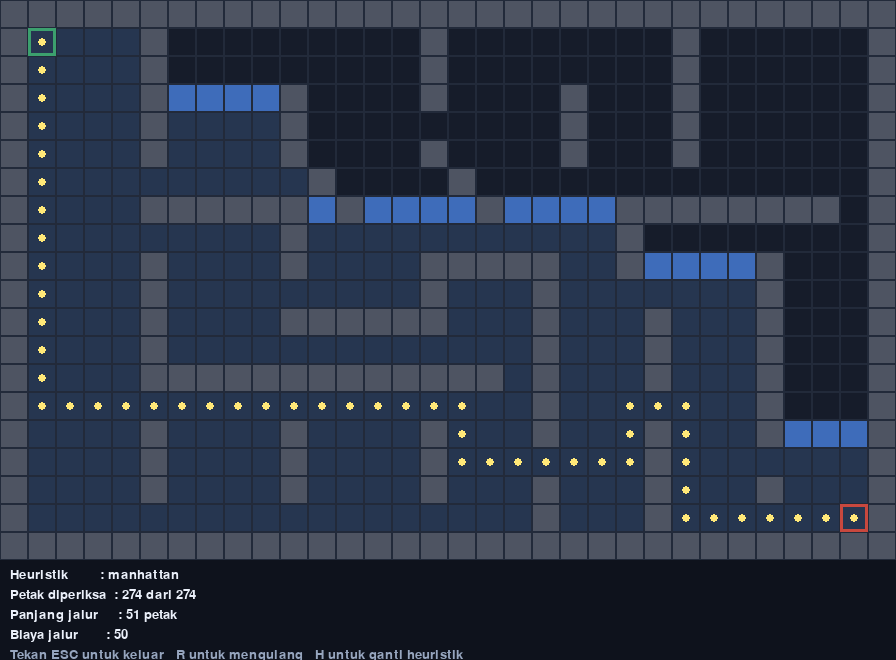
\includegraphics[width=0.62\linewidth]
      {../buku_ajar/chapters/10/figures/pencarian-manhattan.png}
    {\scriptsize\bfseries Manhattan: 274 petak\par}
  \end{column}
  \begin{column}{0.49\textwidth}
    \centering
    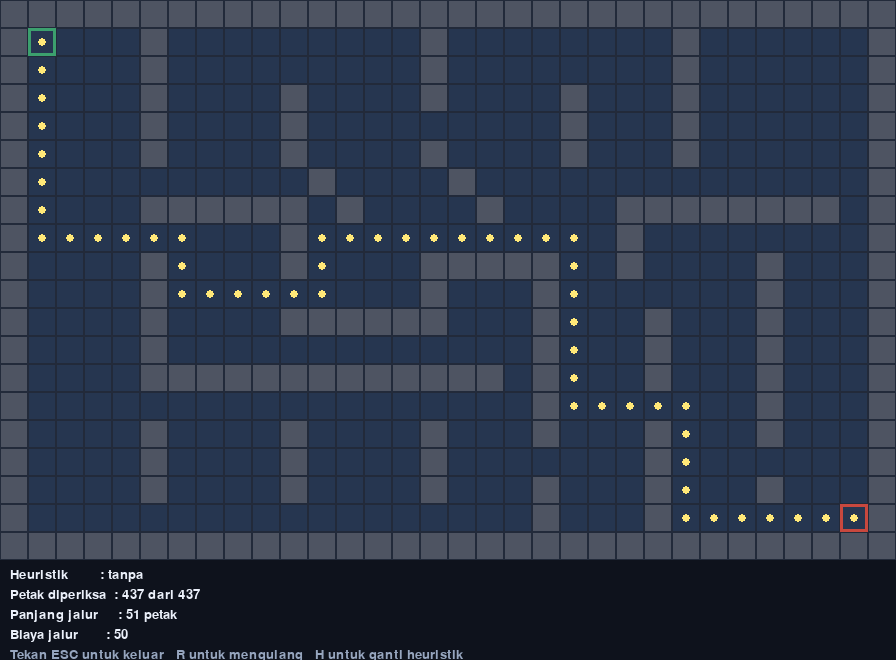
\includegraphics[width=0.62\linewidth]
      {../buku_ajar/chapters/10/figures/pencarian-dijkstra.png}
    {\scriptsize\bfseries Dijkstra: 437 petak\par}
  \end{column}
\end{columns}
\vspace{0.10cm}
\begin{kotak}
Petak biru gelap adalah petak yang telah diperiksa, biru terang adalah petak
yang menunggu diperiksa, dan bulatan kuning adalah jalur yang ditemukan.
Keduanya bukan hiasan, melainkan tangkapan layar dari program yang Anda tulis
sendiri melalui pilihan \texttt{-{}-simpan-gambar}.
\end{kotak}
\end{frame}

% ========================================================= bagian 4
\section{Merekonstruksi dan Memvisualisasikan Jalur}
\sectionframe{04}{Merekonstruksi dan Memvisualisasikan Jalur}
  {Tabel asal, penelusuran mundur, dan pemeriksaan keabsahan}

\begin{frame}{Menyimpan Asal Setiap Petak}
\awalan{Pencarian yang berhasil menemukan tujuan baru menyelesaikan separuh
pekerjaan. Separuhnya lagi adalah mengetahui jalan menuju ke sana.}
\begin{itemize}
  \item Selama pencarian, program menyimpan dari petak mana setiap petak
        ditemukan. Simpanan itu disebut tabel asal
        (\emph{came\_from}), dan bentuknya kamus yang memetakan sebuah petak
        ke petak sebelumnya.
  \item Cukup satu baris, \texttt{asal[tetangga\_petak] = sekarang}, untuk
        merekonstruksi jalur.
  \item Setiap petak hanya memiliki satu asal, yaitu petak yang dilalui untuk
        mencapainya dengan biaya termurah.
  \item Apabila jalur yang lebih murah ditemukan kemudian, nilai asalnya
        ditimpa, sehingga tabel itu selalu menyatakan jalur termurah yang
        diketahui saat itu.
\end{itemize}
\vspace{0.12cm}
\begin{kotak}
Tanpa tabel asal, pencarian tetap menemukan tujuan tetapi tidak dapat
menyebutkan petak mana saja yang dilalui. Tabel itu murah disimpan dan menjadi
satu-satunya catatan yang diperlukan untuk rekonstruksi.
\end{kotak}
\end{frame}

\begin{frame}[fragile]{Menelusuri Kembali dari Tujuan}
\awalan{Jalur diperoleh dengan menelusuri tabel asal dari titik tujuan mundur
ke titik awal, lalu membalik urutannya.}
\lstinputlisting[language=Python,firstline=203,lastline=210]
  {../buku_ajar/code/python/ch10_astar.py}
\kodejelas{Penelusuran berhenti ketika asalnya bernilai \texttt{None}, yaitu
tanda bahwa petak itu adalah titik awal. Hasilnya berupa daftar petak dari
awal ke tujuan, sehingga dapat langsung dipakai NPC sebagai rangkaian tujuan
yang harus dilaluinya satu per satu.}
\begin{peringatan}
Pemeriksaan \texttt{if tujuan in asal} perlu dilakukan lebih dahulu. Apabila
tujuan tidak dapat dicapai, misalnya karena terkurung dinding, tabel asal
tidak memuat tujuan, dan penelusuran tanpa pemeriksaan itu akan berputar tanpa
henti atau menimbulkan kesalahan.
\end{peringatan}
\end{frame}

\begin{frame}{Memeriksa Jalur dan Memvisualisasikan Pencarian}
\awalan{Pemeriksaan jalur itu murah dan menangkap kesalahan yang berasal dari
peta atau dari rekonstruksi.}
\begin{columns}[T,onlytextwidth]
  \begin{column}{0.47\textwidth}
    {\fontsize{7}{8.5}\selectfont\bfseries\color{ubAccent}MEMERIKSA JALUR}\par
    \vspace{0.04cm}
    \begin{itemize}
      \item Apakah jalurnya ada, yaitu tidak kosong?
      \item Apakah jalur dimulai dari titik awal dan berakhir di titik tujuan?
      \item Apakah petaknya bersambung dan tidak menembus dinding?
    \end{itemize}
  \end{column}
  \begin{column}{0.50\textwidth}
    {\fontsize{7}{8.5}\selectfont\bfseries\color{ubAccent}MENGGAMBAR PENCARIAN}\par
    \vspace{0.04cm}
    \begin{itemize}
      \item Petak yang telah diperiksa (biru gelap) dan yang menunggu
            diperiksa (biru terang).
      \item Petak yang sedang diperiksa, ditandai bingkai kuning.
      \item Jalur yang ditemukan, berupa bulatan kuning.
    \end{itemize}
  \end{column}
\end{columns}
\vspace{0.14cm}
\begin{kotak}
Pencarian diperlihatkan langkah demi langkah, beberapa petak setiap bingkai,
sehingga penyebarannya dapat diamati. Jumlah petak setiap bingkai diubah
melalui pilihan \texttt{-{}-langkah}.
\end{kotak}
\end{frame}

% ========================================================= bagian 5
\section{Program Pencarian Jalur Lengkap}
\sectionframe{05}{Program Pencarian Jalur Lengkap}
  {Lima bagian program, inti pencarian, dan keluaran pengukuran}

\begin{frame}{Lima Bagian Program Pencarian Jalur}
\awalan{Program pencarian jalur menyatukan seluruh unsur menjadi satu berkas
yang dapat diamati dan diukur.}
\begin{enumerate}
  \item \textbf{Pembacaan peta} --- \texttt{baca\_peta} mengubah gambar huruf
        menjadi himpunan dinding, titik awal, dan titik tujuan.
  \item \textbf{Penentuan tetangga} --- \texttt{tetangga} mengembalikan petak
        yang bersebelahan dan dapat dilalui.
  \item \textbf{Ukuran heuristik} --- tiga fungsi kecil, yaitu
        \texttt{jarak\_manhattan}, \texttt{jarak\_euclidean}, dan
        \texttt{tanpa\_perkiraan}.
  \item \textbf{Pencarian} --- \texttt{cari\_jalur} menjalankan A* dengan
        antrean prioritas, lalu merekonstruksi jalurnya.
  \item \textbf{Pemeriksaan dan penggambaran} --- \texttt{periksa\_jalur}
        memeriksa keabsahan jalur, sedangkan \texttt{gambar\_peta} menampilkan
        keadaan pencarian.
\end{enumerate}
\vspace{0.12cm}
\begin{kotak}
Pemisahan itu membuat setiap bagian dapat diganti tanpa mengganggu yang lain.
Mengubah arah gerak hanya menuntut perubahan pada \texttt{tetangga}; mengganti
heuristik hanya menuntut penambahan satu fungsi kecil.
\end{kotak}
\end{frame}

\begin{frame}[fragile]{Memasukkan Tetangga ke Antrean Prioritas}
\awalan{Inti pencarian terletak pada pemeriksaan setiap tetangga dari petak
yang baru saja dikeluarkan dari antrean.}
\lstinputlisting[language=Python,firstline=195,lastline=201]
  {../buku_ajar/code/python/ch10_astar.py}
\kodejelas{\texttt{biaya\_baru} adalah biaya sejauh ini ditambah satu langkah.
Nilai \texttt{perkiraan} adalah $g + h$ untuk petak tetangga, dan
\texttt{asal} mencatat dari mana petak itu dicapai.}
\vspace{0.08cm}
\begin{kotak}
Petak dimasukkan kembali setiap kali ditemukan jalur yang lebih murah menuju
ke sana. Cara itu lebih sederhana daripada memperbarui isi antrean, dan
hasilnya tetap benar.
\end{kotak}
\end{frame}

\begin{frame}[fragile]{Keluaran \texttt{-{}-bandingkan} dan Percobaan}
\begin{lstlisting}[language={},numbers=none,
  basicstyle=\ttfamily\scriptsize\color{ubCodeText}]
  Heuristik  Diperiksa   Jalur   Biaya  Temuan
--------------------------------------------------
  manhattan        274      51      50       0
  euclidean        353      51      50       0
      tanpa        437      51      50       0
--------------------------------------------------
\end{lstlisting}
\kodejelas{Kolom \emph{Temuan} menyatakan banyaknya masalah yang ditemukan
oleh pemeriksaan jalur. Nilainya nol pada ketiga baris, yang berarti ketiga
jalur itu bersambung, dimulai dari titik awal, berakhir di titik tujuan, dan
tidak melewati dinding.}
\begin{itemize}
  \item Ubah heuristik melalui \texttt{-{}-heuristic} atau tombol H: bentuk
        penyebaran berubah, sedangkan biaya jalurnya tetap.
  \item Pindahkan \texttt{G} atau tambah dinding: jalur menyesuaikan; bila
        tujuan terkurung, jalurnya kosong dan keadaan itu harus ditangani.
  \item Gandakan \texttt{jarak\_manhattan}: pencarian lebih cepat, tetapi
        biaya jalur dapat lebih besar daripada 50.
\end{itemize}
\end{frame}

% ========================================================= bagian 6
\section{Yang Belum Ada pada Pencarian Ini}
\sectionframe{06}{Yang Belum Ada pada Pencarian Ini}
  {Dari jalur yang ditemukan menuju NPC yang benar-benar menempuhnya}

\begin{frame}{Tiga Persoalan yang Belum Dijawab}
\awalan{Program pada bab ini mencari jalur dan memperlihatkannya, tetapi belum
ada NPC yang menempuh jalur itu.}
\begin{enumerate}
  \item \textbf{Kapan pencarian dijalankan.} Pencarian tidak dapat dijalankan
        setiap bingkai untuk setiap NPC, sebab biayanya terlalu besar.
        Keputusan tentang kapan pencarian perlu diulang merupakan inti materi
        berikutnya.
  \item \textbf{Rintangan yang bergerak.} Peta pada bab ini tetap. Apabila ada
        benda yang berpindah menutupi jalan, jalur yang sudah dihitung dapat
        menjadi tidak berlaku di tengah jalan.
  \item \textbf{Jalur yang ditempuh benda.} Jalur berupa rangkaian petak,
        sedangkan benda bergerak dengan kecepatan dalam piksel per detik.
        Perlu aturan untuk menentukan kapan sebuah petak dianggap sudah
        dicapai.
\end{enumerate}
\vspace{0.12cm}
\begin{kotak}
Penghubungan pencarian dengan NPC adalah pekerjaan Materi 9, dan penghubungan
itu tidak sesederhana menambahkan beberapa baris. Ketiga persoalan di atas
harus dijawab sebelum NPC dapat mengejar pemain dengan rute memutar.
\end{kotak}
\end{frame}

\begin{frame}{Bentuk Peta yang Lebih Rumit}
\awalan{Tiga bentuk pengembangan berikut lazim dipakai pada permainan yang
sesungguhnya.}
\begin{itemize}
  \item \textbf{Delapan arah}, sehingga benda dapat bergerak diagonal.
        Heuristiknya harus disesuaikan agar tidak melebihkan jarak; jarak
        Manhattan tidak lagi memenuhi syarat itu.
  \item \textbf{Peta berbiaya berbeda}, misalnya jalan berbatu yang lebih
        lambat dilalui. Pencariannya tidak berubah, sebab A* memang sudah
        memperhitungkan biaya sisi; yang berubah hanyalah nilai biaya pada
        fungsi penentuan tetangga.
  \item \textbf{\emph{NavMesh}}, yaitu peta jalur berupa rangkaian bidang yang
        menutupi daerah yang dapat dilalui, bukan rangkaian petak. Cara itu
        lebih tepat untuk peta tiga dimensi.
\end{itemize}
\vspace{0.12cm}
\begin{kotak}
Pemahaman tentang NavMesh pada dasarnya adalah pemahaman yang sama dengan yang
Anda peroleh pada bab ini: simpul, sisi, biaya, dan pencarian. Perbedaannya
terletak pada bentuk simpulnya, yaitu bidang segitiga alih-alih petak, dan
pada kenyataan bahwa pencariannya dilakukan oleh mesin.
\end{kotak}
\end{frame}

\begin{frame}{Ringkasan Perkembangan}
\awalan{Bab ini melengkapi lapisan navigasi. Setelah bab ini, kedua lapisan
sudah tersedia: lapisan keputusan pada FSM dan lapisan navigasi pada A*.}
{\scriptsize
\renewcommand{\arraystretch}{1.14}
\begin{tabularx}{\textwidth}{@{}>{\centering\arraybackslash}p{1.8cm}
    >{\raggedright\arraybackslash}p{5.2cm} X@{}}
\toprule
\textbf{Materi} & \textbf{Yang ditambahkan} & \textbf{Akibatnya} \\
\midrule
Materi 9 & Penghubungan dengan mesin keadaan, penyimpanan jalur, dan
pengulangan pencarian secara berkala &
NPC mengejar dengan rute memutar, dan biaya pencariannya diatur agar tetap
ringan. \\
Materi 10--11 & \emph{NavMesh} pada Unity &
Pencarian jalur diserahkan kepada mesin, sedangkan kode Anda mengatur tujuan,
luas jangkauan, dan tingginya rintangan. \\
\bottomrule
\end{tabularx}}
\vspace{0.16cm}
\begin{kotak}
Materi 9 menghubungkan lapisan keputusan dengan lapisan navigasi, dan di
sanalah NPC yang sebenarnya terbentuk. Mini Proyek AI menuntut keduanya bekerja
bersama pada skenario labirin dan rintangan dinamis sederhana.
\end{kotak}
\end{frame}

% --------------------------------------------------------- aktivitas
\begin{frame}{Aktivitas di Kelas \textperiodcentered\ Praktikum 08}
\awalan{Pengalaman belajar minggu 8 pada RPS, dikerjakan berurutan di kelas lalu
diselesaikan di rumah.}
\begin{enumerate}
  \item Jalankan \texttt{ch10\_astar.py}, lalu amati penyebaran pencarian dari
        titik awal menuju titik tujuan.
  \item Jalankan \texttt{-{}-bandingkan}, catat tabel ketiga heuristik, lalu
        bandingkan banyaknya petak yang diperiksa.
  \item Jalankan \texttt{-{}-heuristic manhattan}, tekan H untuk berganti
        heuristik, dan amati perubahan bentuk penyebarannya.
  \item Pindahkan huruf \texttt{G}, tambahkan dinding, lalu buat satu keadaan
        yang membuat tujuan tidak dapat dicapai.
  \item Simpan tangkapan layar dengan \texttt{-{}-simpan-gambar} dan sertakan
        gambar itu pada laporan praktikum.
  \item Gandakan hasil \texttt{jarak\_manhattan}, jalankan
        \texttt{-{}-bandingkan}, lalu jelaskan akibatnya terhadap biaya jalur.
\end{enumerate}
\vspace{0.10cm}
{\footnotesize\color{ubAccent}\itshape Rincian lengkap: Praktikum 08 pada Bab X
buku ajar. Simpan pekerjaan ke repositori Git dengan pesan yang menerangkan
isinya.}
\end{frame}

% --------------------------------------------------------- rangkuman
\begin{frame}{Rangkuman}
\begin{itemize}
  \item Peta berpetak diubah menjadi graf dengan tiga aturan: petak kosong
        menjadi simpul, petak bersebelahan menjadi sisi, dan biaya setiap sisi
        bernilai satu.
  \item BFS memeriksa menurut banyaknya langkah; Dijkstra memeriksa menurut
        biaya sejauh ini $g$; A* memakai $f = g + h$, sehingga pencariannya
        terarah. Dijkstra adalah A* dengan $h$ bernilai nol.
  \item Tepi pencarian berupa antrean prioritas dari modul \texttt{heapq}.
        Sebuah petak dapat masuk antrean lebih dari sekali, dan isi yang sudah
        usang dibuang dengan memeriksa biaya terkini.
  \item Heuristik harus tidak pernah melebihkan jarak. Manhattan dan Euclidean
        memenuhinya untuk gerak empat arah; Manhattan tidak memenuhinya untuk
        gerak delapan arah.
  \item Pada peta bab ini Manhattan memeriksa 274 petak, Euclidean 353 petak,
        dan Dijkstra 437 petak, sedangkan biaya jalurnya sama, yaitu 50.
  \item Jalur direkonstruksi dari tabel asal dengan menelusuri mundur dari
        tujuan lalu membalik urutannya; keadaan tujuan yang tidak dapat dicapai
        harus ditangani.
\end{itemize}
\end{frame}

% --------------------------------------------------------- cek
\begin{frame}{Cek Pemahaman}
\begin{enumerate}
  \item Mengapa BFS tidak memadai ketika biaya sisi berbeda-beda, walaupun ia
        menjamin jalur dengan langkah paling sedikit?
  \item Sebuah petak berjarak delapan langkah dari titik awal dan tiga satuan
        Manhattan dari titik tujuan. Hitunglah $f$-nya, lalu jelaskan mengapa
        nilai itu menentukan urutan pemeriksaannya.
  \item Manhattan memeriksa 274 petak sedangkan Dijkstra 437 petak, tetapi
        biaya jalurnya sama. Jelaskan mengapa demikian, dan apa yang terjadi
        bila heuristiknya digandakan?
\end{enumerate}
\vspace{0.35cm}
{\footnotesize\color{ubMuted}\itshape Jawab tanpa membuka catatan, lalu
bandingkan dengan pasangan di sebelah Anda.}
\end{frame}

% --------------------------------------------------------- penutup
\penutup{Tugas Praktikum 08; Kuis 2 (Materi 6--7)}
  {\hyphenpenalty=10000 \exhyphenpenalty=10000 \sloppy
   Materi 9 menghubungkan lapisan keputusan (FSM) dengan lapisan navigasi
   (A*): \mbox{\emph{state chase}} memanggil A* dan melakukan
   \mbox{\emph{repath}} berkala,
   lalu perilaku NPC diuji pada labirin dan rintangan dinamis sederhana
   melalui Mini Proyek AI.}

\end{document}
